
%%%%%%%%%%%%%%%%%%%%%%%%%%%%%%%%%%%%%%%%%%%%%%%%%%%%%%%%%%%%%%%%%%%%
%%%%%%%%%%%%%%%%%%%%%%%%%%%%%%%%%%%%%%%%%%%%%%%%%%%%%%%%%%%%%%%%%%%%
a\chapter{GENFORM tool} \label{metadata}



% ==================================================================
\section{What is GENFORM ?} \label{genform}

GENFORM is a WebObs integrated tool that allows to create \wo{form}. GENFORM can generates new \wo{form} by reading a configuration file (based on the key|value model) with a special syntax. Each \wo{form} is then associated to a table in a database called WEBOBSFORMS.db. Each table of the database contains data based on the following scheme :

\begin{center}
	\begin{tabular}{c c c}
		\hline
		\textit{Name} & \textit{Type} & \textit{Commentaire} \\
		\hline
		id & name & unique \\
		trash & boolean & True = bin	\\
		node & text & ID WebObs of the associated \wo{node} \\
		edate & datetime & date and time end of measurement/collection/sampling \\
		edate_min & datetime & uncertainty date and time end of measurement \\
		sdate1 & datetime & date and time start of measurement/collection/sampling \\
		sdate1_min & datetime & uncertainty date and time end of measurement \\
		users & text & WebObs ID of the operator (authorized list) \\
		input01 & text & data n°1 \\
		input02 & text & data n°2 \\
		... & text & data n°... \\
		comment & text \\
		tsupd & timestamp & last edit timestamp \\
		userupd & text & last edit user ID \\
		\hline
	\end{tabular}
\end{center}

Once a \wo{form} is created through GENFORM, the given \wo{form} works like a normal \wo{form} in WebObs.

\section{Creation of a \wo{form}}

To create a new \wo{form} using GENFORM, you have to go in the \wo{grid} menu list and click on the pencil next to \textbf{Raw Data}. Then, you have to chose a name for the FORM and select a template that will be used to help you through the creation process. Currently, 3 templates exist : 

\begin{list}
	\item GENFORM: the most basic template that shows you all the different types of inputs that you can use in GENFORM
	\item EAUX: a template based on the old EAUX \wo{form} used for the water chemistry
	\item GAZ: a template based on the old GAZ \wo{form} used for the gas chemistry
\end{list}

\begin{figure}[!h]
	\centering
	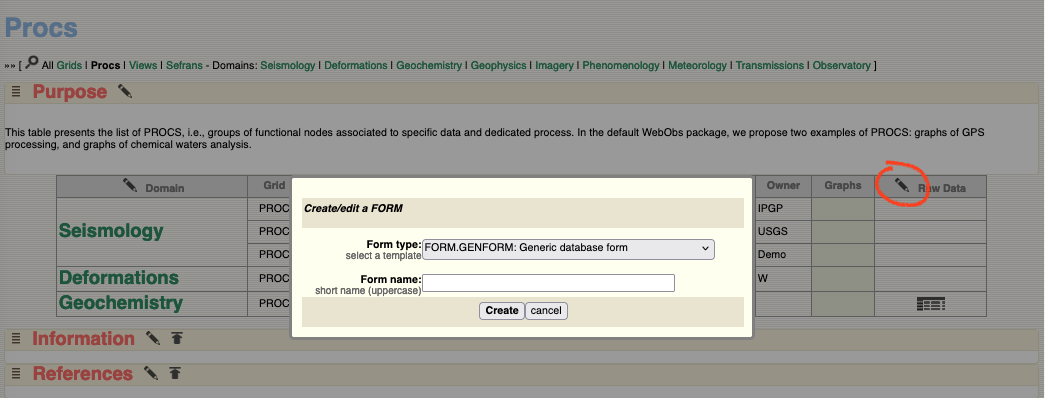
\includegraphics[width=\textwidth]{figures/GENFORM_creation.png}
	\caption{Chose a name and a template and click on Create.}
\end{figure}

If you want to edit a \wo{form}, you just need to go in the GENFORM creation menu and write the name of the \wo{form} you want to edit, no matter the template which is selected.

\section{The GENFORM language}

Each GENFORM is formed of COLUMNS. Each COLUMN contains FIELDSETS. Each FIELDSET contains INPUTS. An INPUT has a NAME, a UNIT and a TYPE. 3 TYPES exist for the moment:

\begin{list}
	\item formula, which allows to make simple mathematical operations between the different INPUTS
	\item list, which allows to use a configuration file to create select input in the form
	\item text (work in progress)
\end{list}

Each FIELDSET has a NAME, a number of COLUMNS and the NAME of the INPUTS you to display in each COLUMN. Each COLUMN have a list of the FIELDSETS you want to display in each COLUMN.

Finally, the configuration file of the \wo{form} has a NAME, that you have chosen at the creation of the \wo{form}, a BANG, which is the begininng year of the dataset associated to the \wo{form}, a title, to display in the \wo{grid} form, column and fieldset numbers and a STARTING_DATE key which is a boolean that allows GENFORM to display or not display a starting date when filling a record form.

